\documentclass[a4paper,12pt]{report}
\usepackage{fullpage}
\usepackage{amsmath}
\usepackage{fancyhdr}
\usepackage{lastpage}
\usepackage{chngcntr}
\usepackage{changepage}
\usepackage{graphicx}
\usepackage{lipsum}
\usepackage{color, soul}
\usepackage{tabularx}
\usepackage{listings}
\usepackage{courier}
\pagestyle{fancy}
\fancyhf{}
\setlength{\headheight}{40pt}
\setlength{\headsep}{0.2in}

\lhead{4-16-2019}
\chead{EECS 649 Homework 9}
\rhead{Cameron Kientz \quad \thepage/\pageref{LastPage}}

\newcounter{problem}
\newenvironment{problem}[2][]{
    \noindent
	% \begin{minipage}{\textwidth}
    \refstepcounter{problem}
    \noindent
    \textbf{\underline{Problem~\theproblem#1}} \bigskip\newline
    \textbf{#2} \bigskip
    \begin{adjustwidth}{1em}{}
    }{\end{adjustwidth}\noindent\rule{\textwidth}{0.4pt}\bigskip
	% \end{minipage}
	}

\newcounter{subproblem}
\counterwithin{subproblem}{problem}
\newenvironment{subproblem}[2][]{
	\begin{minipage}{\textwidth}
    \refstepcounter{subproblem}\textbf{\underline{Part~\alph{subproblem}#1}}
    \textbf{#2} \bigskip
    \begin{adjustwidth}{0.5em}{}
    }{\end{adjustwidth}\bigskip
	\end{minipage}
	}

\lstset{
   basicstyle=\fontsize{8}{5}\selectfont\ttfamily,
   language=Python
}

%%PROBLEM #%%
% \begin{problem}{Questions words?}
%     \begin{subproblem}{Subquestion words}
%         Answer words
%     \end{subproblem}
% \end{problem}

%%PROBLEM #%%
% \begin{problem}{Questions words?}
%     Answer words
% \end{problem}


\begin{document}

%PROBLEM 1%%
\begin{problem}{Tickets to a lottery cost \$1. There are two possible prizes: a \$10 payoff with probabil-ity 1/50, and a \$1,000,000 payoff with probability 1/2,000,000. 
What is the expected mone-tary value of a lottery ticket? When (if ever) is it rational to buy a ticket? Be precise—show anequation involving utilities. You may assume 
current wealth of \$kand thatU(Sk)=0.Youmay also assume thatU(Sk+10)=10×U(Sk+1), but you may not make any assumptionsaboutU(Sk+1,000,000).  Sociological studies show that 
people with lower income buy a dis-proportionate number of lottery tickets. Do you think this is because they are worse decisionmakers or because they have a different 
utility function? Consider the value of contemplating the possibility of winning the lottery versus the value of contemplating becoming an actionhero while watching an 
adventure movie.}
    Answer words
\end{problem}

%PROBLEM 2%%
\begin{problem}{In  1713,  Nicolas  Bernoulli  stated  a  puzzle,  now  called  the  St.  Petersburg  paradox,which works as follows.   You have the opportunity  to play 
a game in which a fair coin is tossed repeatedly until it comes up heads.  If the first heads appears on the nth toss, you win 2n dollars.}
    \begin{subproblem}{ Show that the expected monetary value of this game is infinite.}
        If n is infinite, then
        \[2(\infty)0.5 = \infty\]
    \end{subproblem}
    \begin{subproblem}{How much would you, personally, pay to play the game?}
        I would pay \$1, so if it lands heads first, I get my money back, after that I can only make a profit
    \end{subproblem}
    \begin{subproblem}{Nicolas’s cousin Daniel Bernoulli resolved the apparent paradox in 1738 by suggestingthat the utility of money is measured on a logarithmic scale 
    (i.e.,U(Sn)=alog2n+b,where S_n is the state of having \$n). What is the expected utility of the game under this assumption?}
        Answer words
    \end{subproblem}
    \begin{subproblem}{What is the maximum amount that it would be rational to pay to play the game, assum-ing that one’s initial wealth is \$k}
        Answer words
    \end{subproblem}
\end{problem}

%PROBLEM 3%%
\begin{problem}{A used-car buyer can decide to carry out various tests with various costs (e.g., kick the tires, take the car to a qualified mechanic) 
    and then, depending on the outcome of the tests, decide which car to buy. We will assume that the buyer is deciding whether to buy car c1, that
    there is time to carry out at most one test, and that t1 is the test of c1 and costs \$50.A car can be in good shape (quality $q^+$) or bad shape (quality $q^{−} $-), 
    and the tests might help indicate what shape the car is in. Car c1 costs \$1,500, and its market value is \$2,000 if it is in good shape; if not, \$700 in 
    repairs will be needed to make it in good shape. The buyer’s estimate is that c1 has a 70\% chance of being in good shape}
    \begin{subproblem}{Calculate the expected net gain from buying c1, given no test.}
        With no test, the expected value will be 
        \[(0.7)(2000 - 1500) + (0.3)(2000 - (1500 + 700) = \$290\]
    \end{subproblem}
    \begin{subproblem}{tests can be described by the probability that the car will pass or fail the test given thatthe car is in good or bad shape. We have the 
        following information: 
        \[P(pass|q^+ = 0.8\]
        \[P(pass|q^- = 0.35\]
        Use Bayes’ theorem to calculate the probability that the car will pass (or fail) its test andhence the probability that it is in good (or bad) shape given each 
        possible test outcome.}
        We need to calculate 
        \[P(q^+|pass) = \frac{(P(pass|q^+)(P(q^+)))}{P(pass)}\]
        \[P(q^-|pass) = \frac{(P(pass|q^-(P(q^-)}{P(pass)}\]
        And we know 
        \[P(q^+) = 0.7\]
        \[P(q^-) = 0.3\]
        \[P(pass|q^+) = 0.8\]
        \[P(pass|q^-) = 0.35\]
        \[P(pass) = (0.8)(0.7) + (0.35)(0.3) = 0.665\]
        So its a simple plug and chug to find:
        \[P(q^+)|P(pass) = \frac{(0.8)(0.7)}{0.665} = 0.842\]
        \[P(q^-)|P(pass) = \frac{(0.35)(0.3)}{0.665} = 0.158\]
    \end{subproblem}
    \begin{subproblem}{Calculate the optimal decisions given either a pass or a fail, and their expected utilities}
        If the test is passed, the utility is:
        \[(P(q^+) |P(pass))(2000 - 1550) + (P(q^-) |P(pass))(2000 - 2250) = 339.47\]
        if it does not pass, then it is:
        \[(P(q^+) |P(pass))(2000 - 1550) + (P(q^-) |P(\neg pass))(2000 - 2250) = 42.53\]
    \end{subproblem}
\end{problem}

%PROBLEM 4%%
\begin{problem}{For the 4×3 world shown  in Figure  17.1,  calculate  which  squares  can  be reached from (1,1) by the action sequence[Up,Up,Right] 
    and with what probabilities.Explain how this computation is related to the prediction task (see Section 15.2.1) for a hidden Markov model.  \newline
    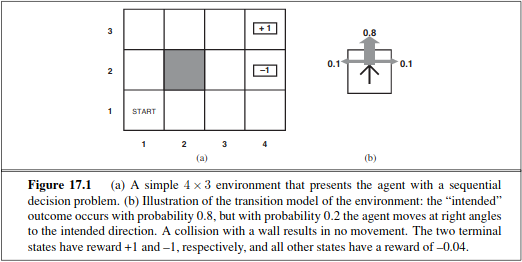
\includegraphics[width=0.6\textwidth]{fig1.png}}
    Answer words
\end{problem}


%PROBLEM 5%%
\begin{problem}{Consider an undiscounted MDP having three states, (1, 2, 3), with rewards−1,−2,0, respectively.  State 3 is a terminal state.  In states 
    1 and 2 there are two possible actions:aandb. The transition model is as follows: \newline
    * In state 1, actionamoves the agent to state 2 with probability 0.8 and makes the agentstay put with probability 0.2. \newline
    * In state 2, actionamoves the agent to state 1 with probability 0.8 and makes the agentstay put with probability 0.2. \newline
    * In either state 1 or state 2, actionbmoves the agent to state 3 with probability 0.1 andmakes the agent stay put with probability 0.9. \newline
    Apply policy iteration, showing each step in full, to determine the optimal policy andthe values of states 1 and 2. Assume that the initial policy has 
    action b in both states.}
    Answer words
\end{problem}


%PROBLEM 6%%
\begin{problem}{Implement the Value-Iteration Algorithm (Figure 17.4 of R\&N) and use it to find the optimal utility values and policy for the 4 x 3 
    world shown in Figure 17.1 of R\&N in the case where $R=−1$(and $gamma=1$). \newline
    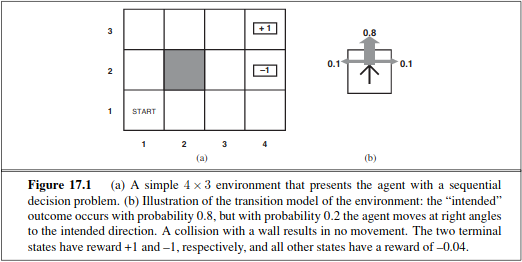
\includegraphics[width=0.6\textwidth]{fig1.png} \newline
    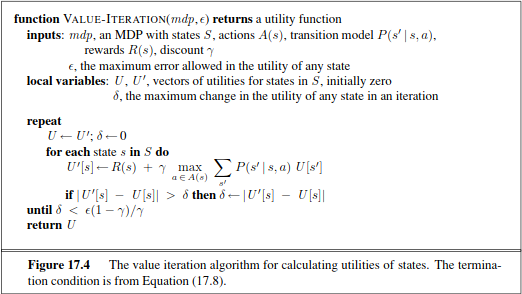
\includegraphics[width=0.6\textwidth]{fig2.png}}
    Answer words
\end{problem}

\end{document}
